%%%%%%%%%%%%%%    general     %%%%%%%%%%%%%% 
\usepackage[utf8]{inputenc}                             % Allows the use of some special characters
\usepackage{amsmath, amsthm, amssymb, amsfonts}         % Nicer mathematical typesetting
%\usepackage[dutch]{babel}  %TODO                         % Changes language of auto-generated text to Dutch 

% Define thuasgreen (color of the Avans logo). Can be changed to drastically change the look of the template
\definecolor{thuasgreen}{RGB}{158, 167, 0}

%%%%%%%%%%%%%%    figures     %%%%%%%%%%%%%% 
\usepackage{graphicx}                                   % Allows the use of \begin{figure} and \includegraphics
\usepackage{float}                                      % Useful for specifying the location of a figure
\usepackage{caption}                                    % Adds additional customization for (figure) captions
\usepackage{subcaption}                                 % Needed to create sub-figures
\usepackage{tikz}

%%%%%%%%%%%%%%     tables     %%%%%%%%%%%%%% 
\usepackage{tabularx}                                   % Adds additional customization for tables
\usepackage{tabu}                                       % Adds additional customization for tables
\usepackage{longtable}                                  % Adds functionality for tables spanning multiple pages
\usepackage{booktabs}                                   % For generally nicer looking tables
\usepackage{colortbl}                                   % Add colors to tables
\usepackage{tabularray}

%%%%%%%%%%%%%%   formatting   %%%%%%%%%%%%%% 
\usepackage[
    margin = 72pt,
    headsep = 26pt,
    footskip = 35pt,
    marginparwidth = 50pt,
    headheight= 20pt,
    showframe = false]{geometry}               % Allows for custom (wider) margins
\usepackage{xcolor}                                     % Defines additional colors and allows user defined colors
\usepackage{appendix}                                   % Any chapter after \appendix is given a letter as index
\usepackage[shortlabels]{enumitem}                      % Adds additional customization for itemize. 
\usepackage{listings}                                   % Makes it possible to add (Java) code to a document

\definecolor{dkgreen}{RGB}{38, 127, 0}
\definecolor{gray}{rgb}{0.5,0.5,0.5}
\definecolor{mauve}{rgb}{0.58,0,0.82}

\lstset{
    language=java,
    showstringspaces=false,
    columns=flexible,
    basicstyle={\ttfamily},
    numbers=left,
    numberstyle=\footnotesize\color{gray!75},
    keywordstyle=\color{thuasgreen},
    commentstyle=\color{dkgreen},
    stringstyle=\color{mauve},
    breaklines=true,
    breakatwhitespace=true,
    tabsize=5,
    % numbersep=-7pt,
    xleftmargin=7pt,
    xrightmargin=7pt,
}

%%%%%%%%%%%%%%  referencing   %%%%%%%%%%%%%%
\usepackage[noabbrev, capitalise, english]{cleveref}      % Easier referencing using \cref{<label>} instead of \ref{}
\usepackage{csquotes}                          % Recommended by biblatex
\usepackage[style=apa, backend=biber]{biblatex}         % Adds a bibliography using APA (causes warning*)
\usepackage{hyperref}                                   % Allows links and makes references and the ToC clickable

% Fixes some APA formatting errors
\DefineBibliographyStrings{dutch}{%
    andothers = {et al\adddot}
}

\DefineBibliographyStrings{dutch}{%
    and = {\&}
}

% Sets up hyperlinks in the document to be colored
\hypersetup{
    colorlinks=true,
    linkcolor=thuasgreen,
    urlcolor=thuasgreen,
    citecolor = thuasgreen
}
\urlstyle{same} % Defines settings for link and reference formatting

% Have reference labels be linked to section (section 3 will have fig. 3.1 etc.)
% \counterwithin{equation}{section} % For equations
% \counterwithin{figure}{section} % For figures
% \counterwithin{table}{section} % For tables

%% TODO: stray packages
\usepackage{richcolorboxes}


%%%%%%%%%%%%%%  Dummy Text   %%%%%%%%%%%%%%
\usepackage{lipsum}
\usepackage{blindtext}
\usepackage{layout}


%%%%%%%%%%%%%%  Temporary packages and code for the front page    %%%%%%%%%%%%%% 

% Give your report a title 
\newcommand\reporttitle{Report\\[2pt] Programming Class}

% Insert module code, name, period number and year (or any other subtitle)
\newcommand\reportsubtitle{
    \textit{Programming Class 24/25}
}

% Insert author and student number here
\newcommand\studentID{
    24097993
}

\newcommand\studentName{
    Kerr Beeldens
}

% Date and location (default: current date and Breda)
\newcommand\placeanddate{
    Bachelor program UXD, THUAS
}

\usepackage[absolute,overlay]{textpos}                  % Allows absolute positioning of text (used by front page)
\usepackage{eso-pic}                                    % Allows absolute positioning of figures (used by front page)
\usepackage{tikz, pgfplots} \pgfplotsset{compat=1.18}   % Useful for drawing images, used for creating the front page
\usetikzlibrary{positioning}                            % Additional library for relative positioning 
\usetikzlibrary{calc}                                   % Additional library for calculating within tikz

% declares layers used by tikz for front-page
\pgfdeclarelayer{background}
\pgfsetlayers{background, main}

\makeatletter
\renewcommand\maketitle{%
    \begin{titlepage}
        \thispagestyle{empty}

        {\sffamily

            \AddToShipoutPicture*{\put(-4,0){
                    \parbox[b][\paperheight]{\paperwidth}{%
                        \vfill
                        \centering
                        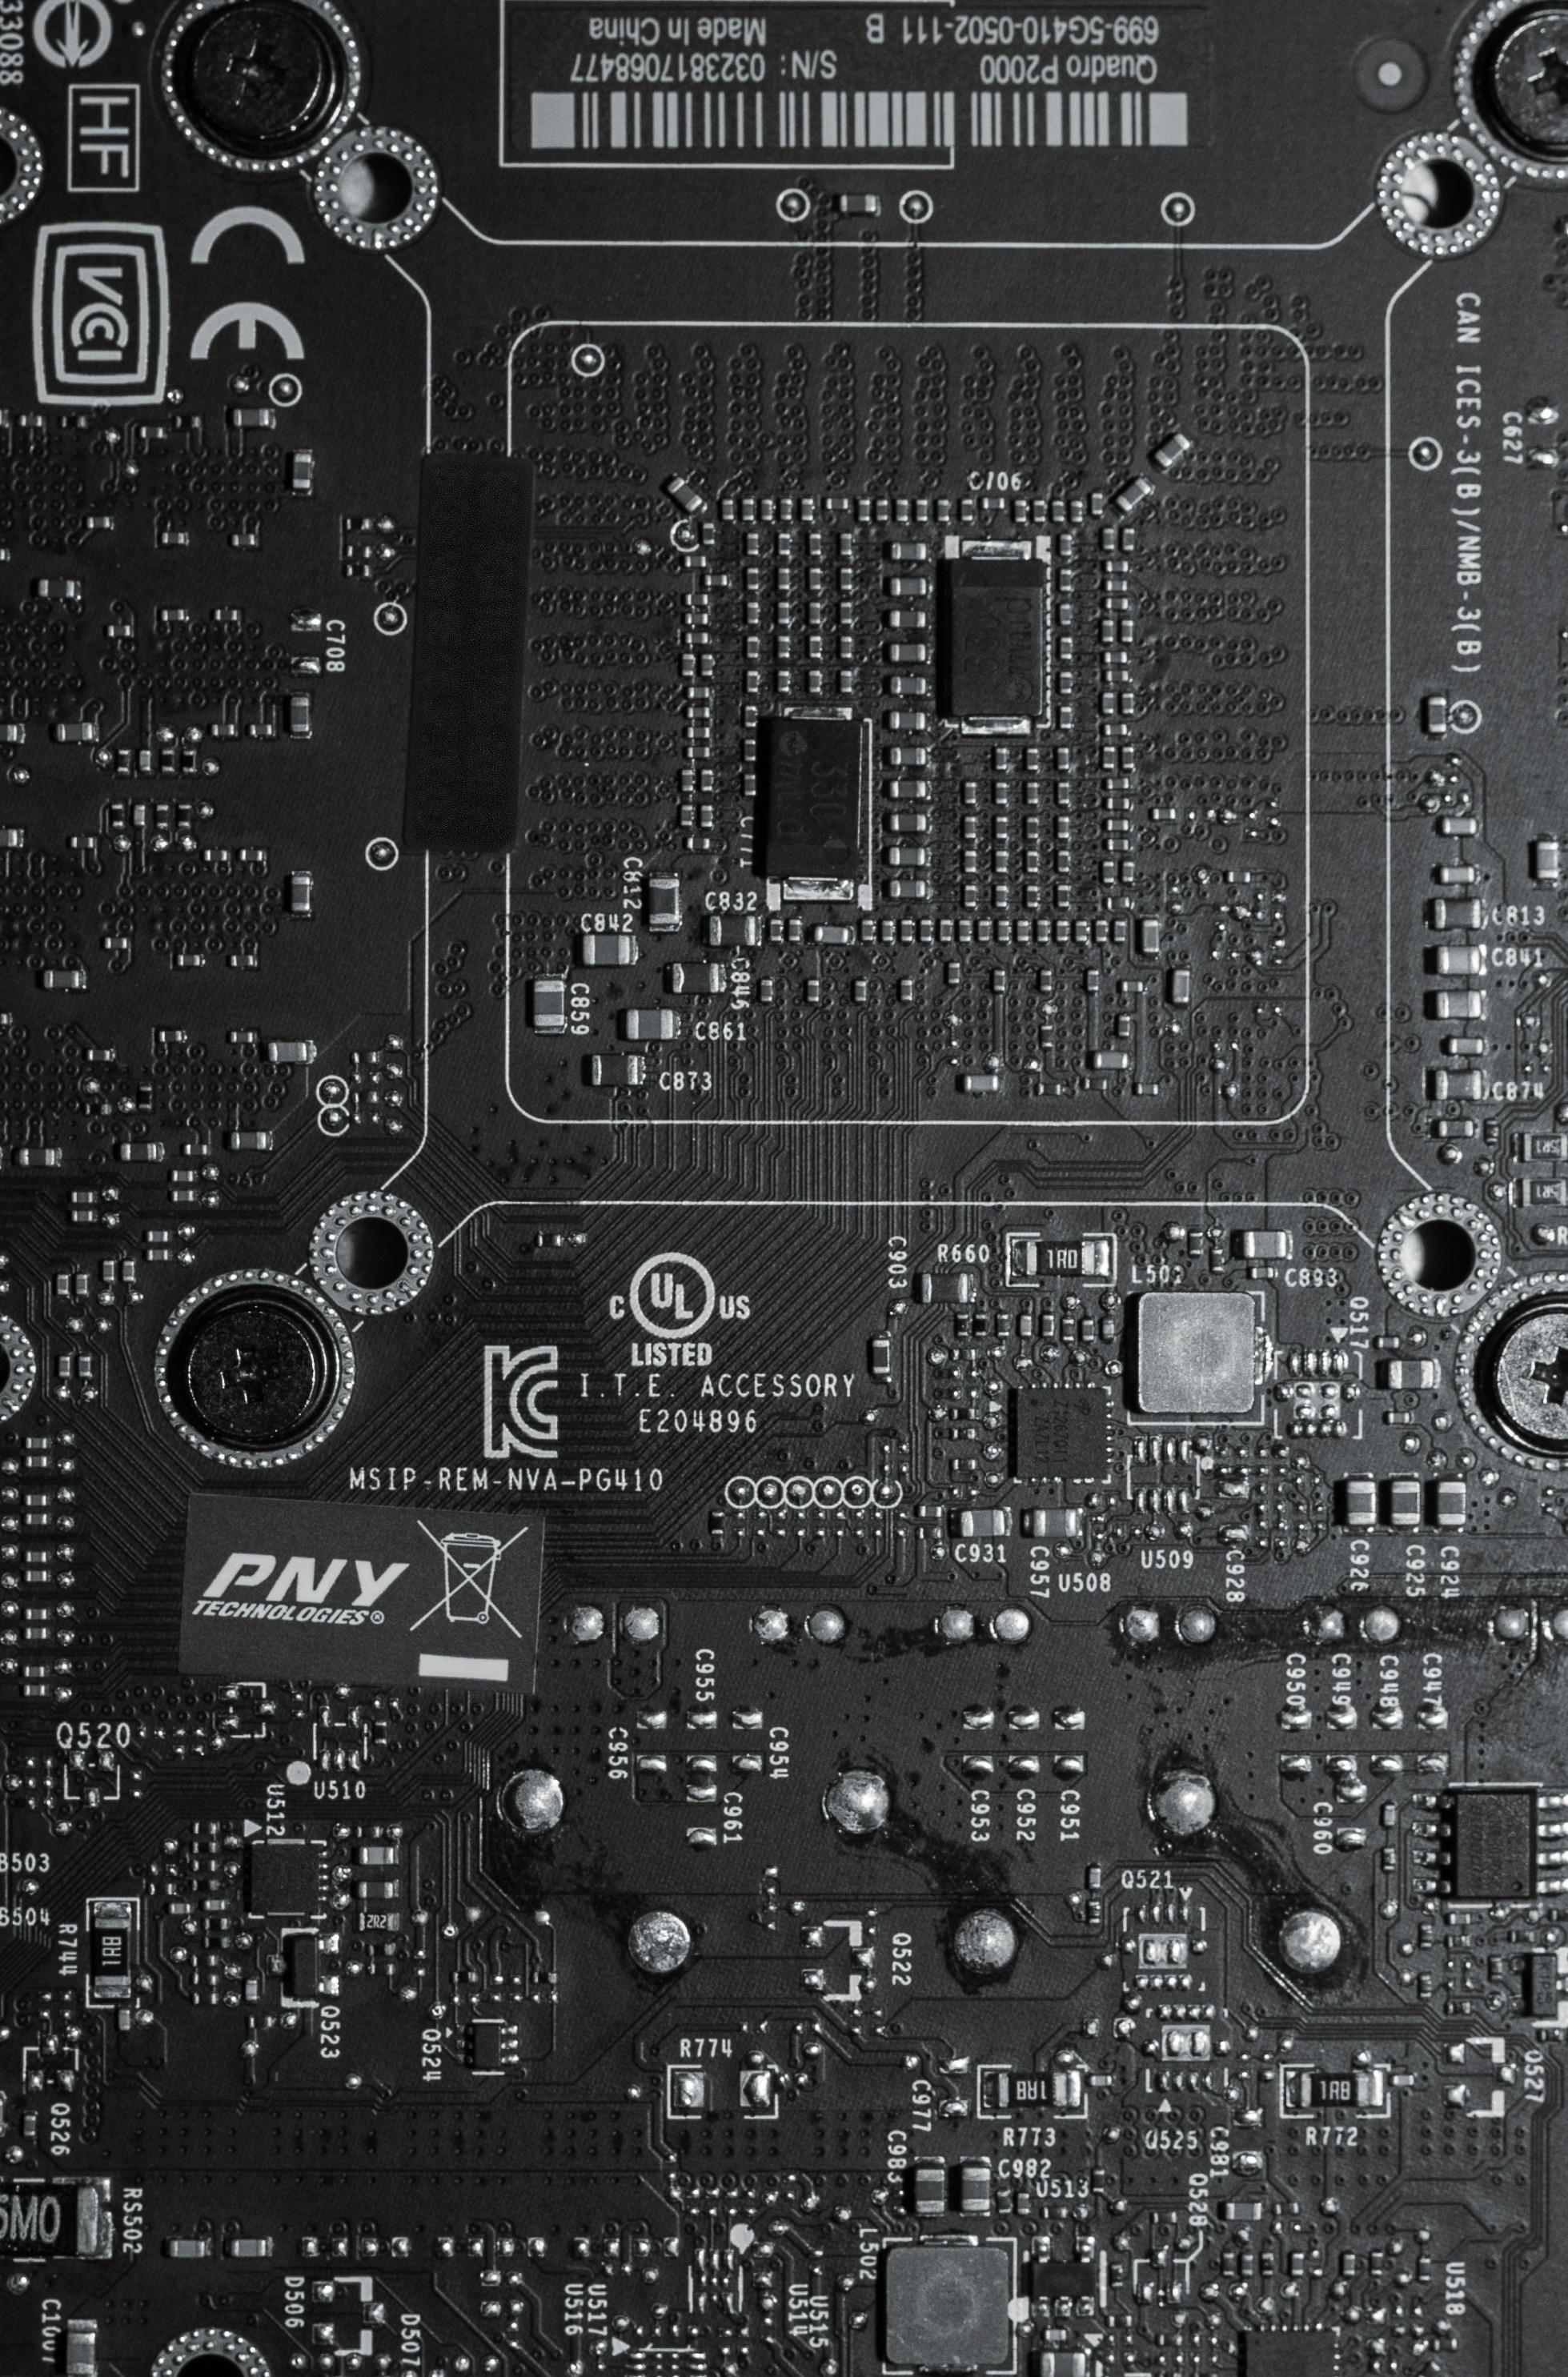
\includegraphics[width=\paperwidth,height=\paperheight]{Figures/0. General/frontpage.jpg}
                        \vfill
                    }}}

            \AddToShipoutPicture*{\put(-4,0){
                    \parbox[b][\paperheight]{\paperwidth}{%
                        \vfill
                        \centering
                        \includegraphics[width=\paperwidth,height=\paperheight]{Figures/0. General/FrontPage.pdf}
                        \vfill
                    }}}

            \begin{textblock*}{8.5cm}(8.5cm, 5.5cm) % {block width} (coords) 
                \Huge\textbf{\reporttitle}\\[2mm]
                \Large \reportsubtitle\\[0mm]
                \placeanddate
            \end{textblock*}

            \begin{textblock*}{6cm}(0cm, 20.75cm) % {block width} (coords) 
                \textblockcolour{headerrule}
                \vspace{3mm}
                \hspace{2mm}
                \Large\textcolor{white}{Student ID: \studentID}
                \vspace{3mm}
            \end{textblock*}


            \begin{textblock*}{7cm}(0cm, 22cm) % {block width} (coords) 
                \textblockcolour{sectionlabel}
                \vspace{3mm}
                \hspace{2mm}
                \Huge\textbf{\textcolor{white}{\studentName}}
                \vspace{3mm}
            \end{textblock*}


            \begin{textblock*}{6.5cm}(0cm, 29cm) % {block width} (coords) 
                \textblockcolour{sectionlabel}
                \vspace{1mm}
                \hspace{2mm}
                \small\textbf{\textcolor{white}{Picture by Albert Stoynov on Unsplash}}
                \vspace{1mm}
            \end{textblock*}

            \begin{tikzpicture}[remember picture]
                % \begin{pgfonlayer}{background}
                %     \node[opacity=0.25,inner sep=0pt,overlay, yshift = -0.25cm] at (9.5,-3.85)
                %     {\includegraphics[width= 0.6 \textwidth] % 0.85 size, 0.25 opacity
                %         {Figures/0. General/THUAS.pdf}};
                % \end{pgfonlayer}
            \end{tikzpicture}
        }
    \end{titlepage}
}
\makeatother

\RequirePackage{fontspec} % TODO: disable if pdflatex

% Set general fonts
\setmainfont{TeX Gyre Pagella}
\setsansfont{TeX Gyre Heros}

% Set colors

\usepackage{xcolor}
\definecolor{headerrule}{RGB}{34, 51, 67}
\definecolor{captionlabel}{RGB}{158, 167, 0}
\definecolor{chapterlabel}{RGB}{34, 51, 67}
\definecolor{sectionlabel}{RGB}{158, 167, 0}
\definecolor{bulletlabel}{RGB}{158, 167, 0}
\definecolor{chaptertoclabel}{RGB}{34, 51, 67}
\definecolor{Avans-red}{RGB}{158, 167, 0}

% Primary colours
\definecolor{richcolorboxtitlebox}{RGB}{158, 167, 0}
\definecolor{richcolorboxtitletext}{RGB}{255, 255, 255}
\definecolor{thuasblue}{RGB}{34, 51, 67}
\colorlet{richcolorboxbodybox}{thuasblue!4}
\definecolor{richcolorboxbodytext}{RGB}{0, 0, 0}

% Questionbox
\colorlet{richquestionboxtitlebox}{richcolorboxtitlebox}
\colorlet{richquestionboxtitletext}{richcolorboxtitletext}
\colorlet{richquestionboxbodybox}{richcolorboxbodybox}
\colorlet{richquestionboxbodytext}{richcolorboxbodytext}

% Cautionbox
\colorlet{richcautionboxtitlebox}{richcolorboxtitlebox}
\colorlet{richcautionboxtitletext}{richcolorboxtitletext}
\colorlet{richcautionboxbodybox}{richcolorboxbodybox}
\colorlet{richcautionboxbodytext}{richcolorboxbodytext}

% Hyperlinkbox
\colorlet{richhyperlinkboxtitlebox}{richcolorboxtitlebox}
\colorlet{richhyperlinkboxtitletext}{richcolorboxtitletext}
\colorlet{richhyperlinkboxbodybox}{richcolorboxbodybox}
\colorlet{richhyperlinkboxbodytext}{richcolorboxbodytext}

% Codebox
\colorlet{richcodeboxtitlebox}{richcolorboxtitlebox}
\colorlet{richcodeboxtitletext}{richcolorboxtitletext}
\colorlet{richcodeboxbodybox}{richcolorboxbodybox}
\colorlet{richcodeboxbodytext}{richcolorboxbodytext}

% Exercisebox
\colorlet{richexerciseboxtitlebox}{richcolorboxtitlebox}
\colorlet{richexerciseboxtitletext}{richcolorboxtitletext}
\colorlet{richexerciseboxbodybox}{richcolorboxbodybox}
\colorlet{richexerciseboxbodytext}{richcolorboxbodytext}